% Source: tex/chapters/ch06/05_ソフトウェアエンジニアリング運用計画.tex
\subsubsection{ソフトウェアとデータの安全性、セキュリティ、完全性、保護、統制}

運用では、情報セキュリティをすべてのサービス活動の中で管理する必要がある。これは、情報の安全性と可用性に関するリスク評価を行い、統制を実施することである。

運用で考えるべき統制には、経営層による情報セキュリティ方針の定義、役割と責任の割当、方針の有効性を監視する責任者、セキュリティ教育、全職員への方針周知、リスク評価と統制実装に関する専門的支援、変更が統制を壊さないことの確認、セキュリティインシデントの報告と対応が含まれる。

DevOpsの発展に伴い、開発運用セキュリティ連携（DevSecOps）が重要になっている。DevSecOpsでは、セキュリティを後工程で追加するのではなく、開発と運用の最初から組み込み、セキュリティ問題の検出と修正をできるだけ早く自動化する。

\begin{figure}[htbp]
\centering
\IfFileExists{assets/generated_figures/ch06/fig-ch06-06.png}{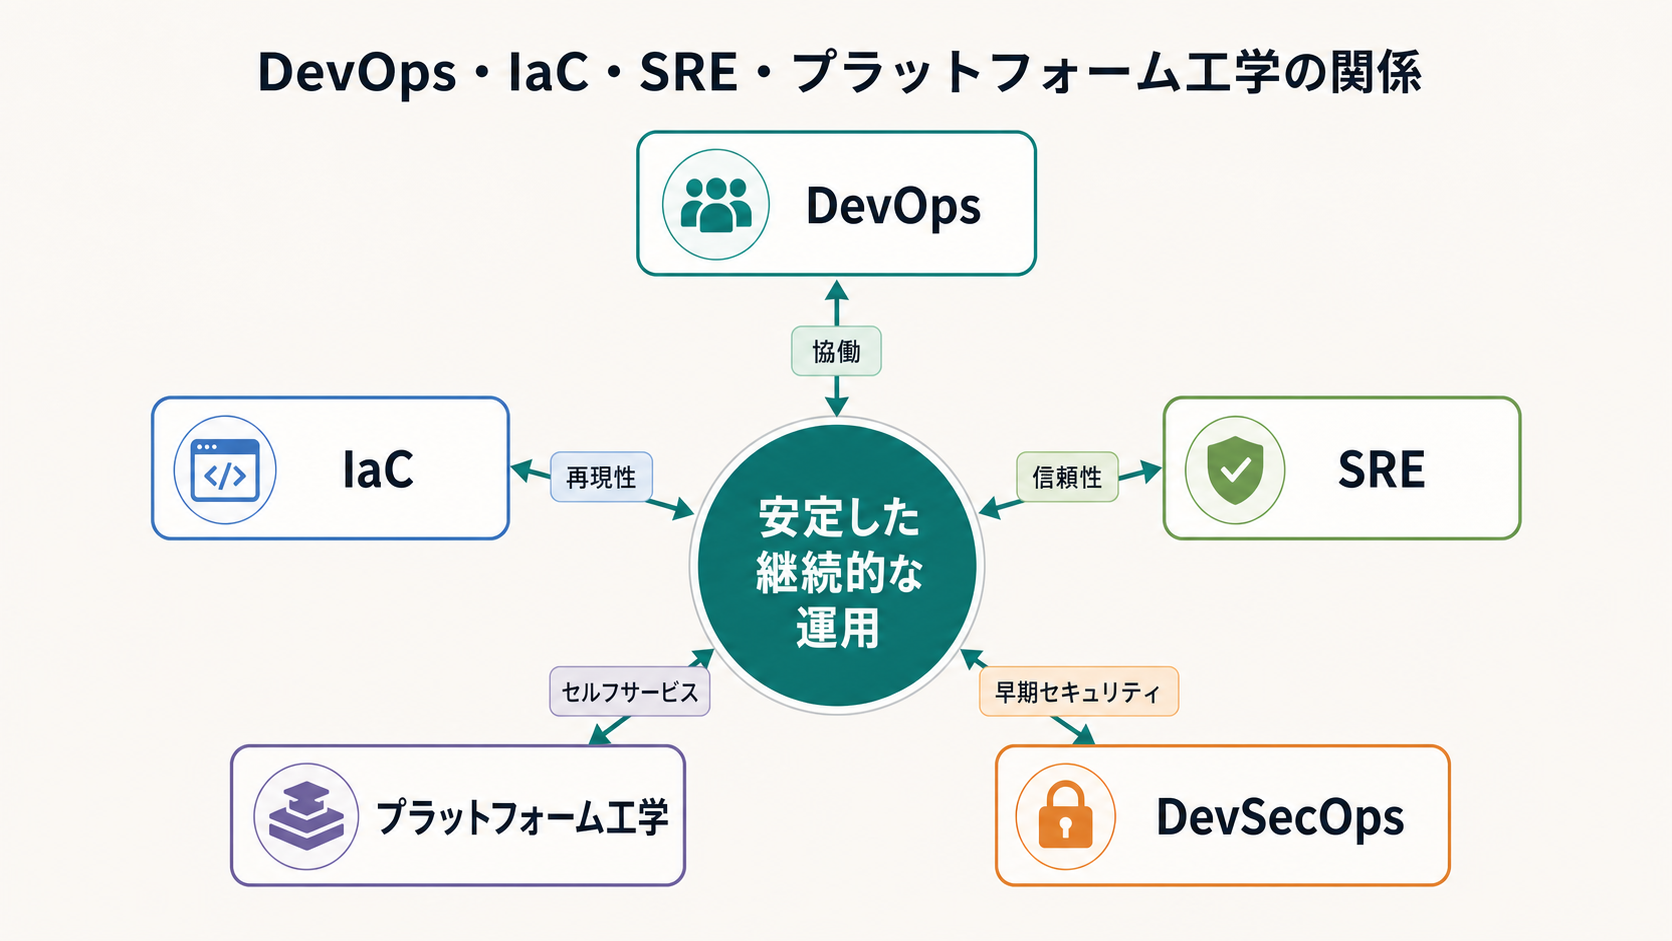
\includegraphics[width=0.96\linewidth]{assets/generated_figures/ch06/fig-ch06-06.png}}{\fbox{\parbox[c][48mm][c]{0.9\linewidth}{\centering 画像生成待ち\\DevOps・IaC・SRE・プラットフォーム工学の関係}}}
\caption{DevOps・IaC・SRE・プラットフォーム工学の関係}
\label{fig:ch06-06}
\end{figure}
